\section*{Introduction}

In 2024, the execution of the \org funded \oldproj demontrated that
ocean model driven \emph{adaptive} robotic exploration, tying targeted
sampling with data assimilated into the model in a virtuous
\emph{sample-assimilate-predict-direct} cycle could enhance model
skill \cite{mendes25,bernacchi26}. The experiment showcased advanced
multi-vehicle adaptive algorithms working with powered low-cost
autonomous underwater vehicles (AUVs) and a stochastic low-latency
model to demonstrate this loop closure. The effort was planned for 3
weeks off the coast of Portugal, in the highly dynamic coastal
bio-geophysically driven environment of the \naz canyon (one of the
longest and deepest submarine canyons in continental Europe).

This study however, had some shortcomings both technical and
logistical. The primary challenges were inclement Fall weather,
unreliable numerical modeling results (hence the fallback to a
statistical model), research vessel failures and leaks in a newly
acquired glider meant to seed the boundary conditions in the
\texttt{HOPS} numerical model. The results as noted in the
publications show promise over the 3-days of data assimilation and
targeted exploration.

In \proj, we propose to build on this effort in the following ways:

\begin{enumerate}

\item Systematically compare between traditional discrete ship-based
  measurements approaches to assimilate data into models with those
  like ours driven by continuous measurements over the diel-cycle

\item Augment and compare assimilative techniques as carried out in
  \oldproj with 3D assimilation over space X time

\item Use multi-variate sampling building on the effort in \oldproj
  which used only temperature as a primary variable to drive
  adaptation 

\item Showcase ensembles of models (both statistical, numerical) and
  compare and contrast model results to drive down averaged model
  uncertainty
  
\item Build on the novel approach to multi-vehicle sampling especially
  with multi-variate statistical optimization for trajectory
  management

\end{enumerate}  

Put together, this advances the science, demonstrates the utility of
robotics to modeling and Physical Oceanography, generates novel ways
to observe the ocean and leverages funded efforts at \orge. Further,
it builds on efforts in the 2005 \textbf{AOSN-II} \cite{ramp09} which
in turn, built on top of \textbf{AOSN} \cite{aosn93} albeit, using low
cost approches to field science, and with a modest budget.

Our objective in \proj is to demonstrate the applicability of
adaptively controlled marine robots in the aerial, surface and
underwater domains, while sampling the upper water-column 'at the
right place and time' driven by ocean models with increasing
predictive skill. In the process, we also plan to mitigate the
shortcomings noted from the earlier experiment, in ways that can
provide for sustained in-water presence of AUVs over a period of 3
weeks to gather valuable data to validate our approach conclusively.
Fig. \ref{fig:block-diag} shows a conceptual view of the proposed
field experiment from \oldproj which continues to be relevant.

\begin{figure}[!]
  \centering
  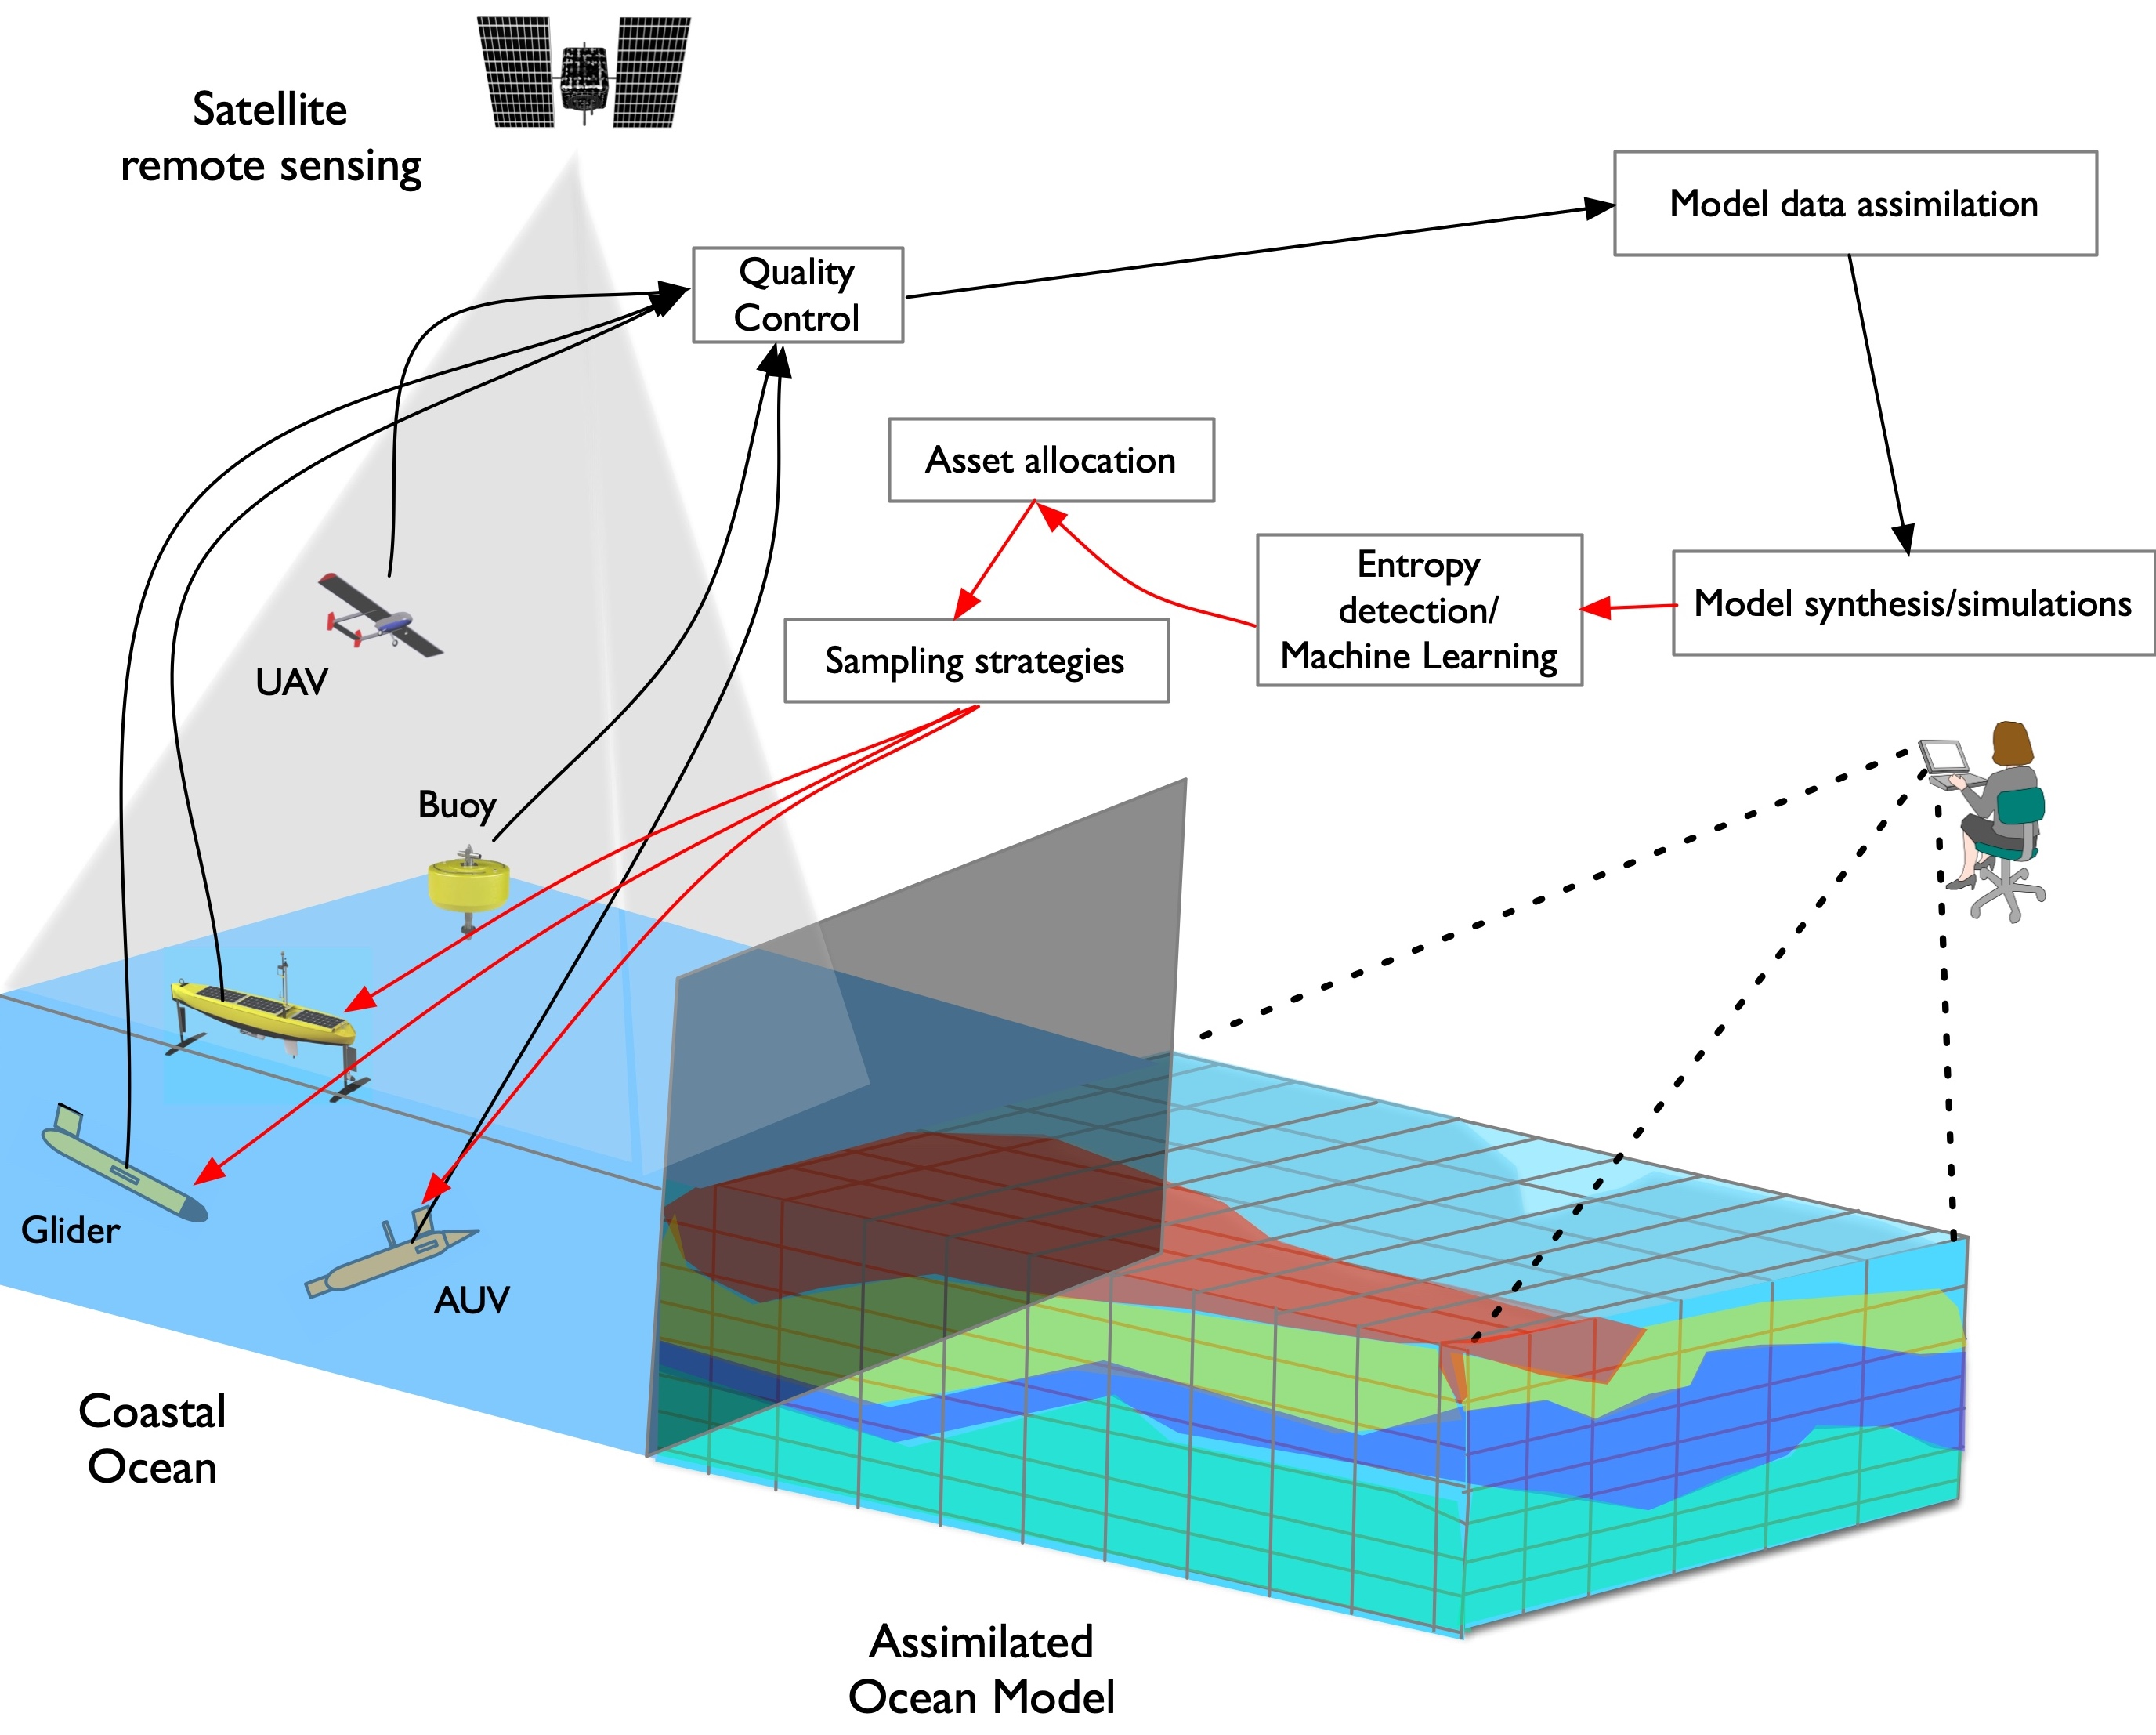
\includegraphics[scale=0.11]{fig/ensemble.jpg}
  \caption{\proj will integrate ocean models with adaptive robotic
    vehicles in the coastal ocean, to increase model skill while
    increasing model accuracy and prediction with a tight loop.}
  \label{fig:block-diag}
\end{figure}

\section*{Motivation}

\proj in an inter-disciplinary field driven experiment spanning the
fields of Physical and Biological Oceanography, Artificial
Intelligence (including Machine Learning), autonomous systems and
Spatial Statistics. It will bring together researchers from these
diverse fields (all of whom have worked with one another) to build on
the integrative aspects of ocean observation especially in a dynamic
coastal environment.  In doing so, the tight integration between model
prediction and assimilation will be enhanced so as to provide
realistic forecasts of a range of bio-physical variables including
temperature, salinity, wind, surface and sub-surface currents and
bio-optical properties. These in turn will be used to
\emph{intelligently target sampling} with robotic vehicles in the air,
surface and underwater domains. Important outcomes of this proposed
project include:

\begin{itemize}[noitemsep,topsep=5pt,parsep=0pt,partopsep=0pt,leftmargin=0.5cm]

\item rapid assessment of environmental state using state of the art
  methods in modeling, control and sampling with minimal human intervention
\item increasing model prediction skill with targeted sampling to
  reduce uncertainty
\item real-time decision support to determine appropriate mix of
  robotic or manned assets (e.g. small boats or research vessel) for
  targeted sampling
\item demonstration of coordinated observations with an ensemble of
  robotic vehicles with minimal human intervention
\end{itemize}

The novelty is in the integrative aspects of this field exercise;
while individual aspects might have been demonstrated in small
experiments (including by members of this team), pulled together this
experiment will leap-frog experimental design, autonomous operations,
assimilation, modeling and prediction in ways not done before.

\section*{Location}
The project will focus on the Bay of Setúbal and the adjacent coastal shelf between Setúbal and Sesimbra. This choice is motivated by the fact that the region combines a semi-enclosed bay, an abrupt coastal mountain system, a narrow and topographically complex shelf, and the nearby Setúbal Canyon, creating a highly heterogeneous environment for testing robotic exploration and short-term coastal predictions. From an operational standpoint, this area is also particularly attractive because it lies within the ZLT Infante D. Henrique, a regulated real-world experimentation area created to test unmanned and other advanced technologies in open-sea conditions and monitored from the Portuguese Navy’s operational experimentation centre in Tróia. The same area regularly hosts the REPMUS exercise, further demonstrating its suitability for complex, multi-platform maritime experimentation. 

The geomorphological setting (Arrábida Chain) justifies treating the region as a topographically and orographically controlled coastal system, where coastline orientation, shelf geometry, and the mountain barrier are expected to modulate local wind exposure, circulation patterns, and the spatial expression of upwelling-related processes. Published studies for the Portuguese west coast show that upwelling-favourable conditions are most consistent in spring and summer and that intense coastal upwelling is strongly shaped by local coastal geometry, with evidence that the upwelling core may separate from the coast depending on shelf structure and the interaction between surface and bottom Ekman layers. Studies in central Portugal further show that complex coastline and bathymetry favour along-slope jets, frontal structures, countercurrents during relaxation, and recirculation cells. In the present project, these mechanisms provide the physical rationale for explicitly testing how local topographic steering alters the recurrence, persistence, and cross-shore organization of upwelling signatures in the Bay of Setúbal–Sesimbra sector.

A second key control is the influence of the Setúbal Canyon, whose head lies about 6 km from the coast at roughly 60 m water depth and which extends for around 150 km down to depths of about 4500 m before merging with the Lisbon canyon system. The canyon therefore introduces a major bathymetric discontinuity very close to the operational area and is expected to affect slope–shelf exchange, local and regional current structure and settings, and the spatial redistribution of suspended material. 

A third process is the role of internal tides and internal waves generated or intensified by complex bathymetry. The available canyon studies for the Lisbon–Setúbal system explicitly identify internal-tide processes as dynamics associated with sediment transport and near-bottom current variability, while broader recent work confirms that internal-wave breaking over sloping topography is a major mechanism for turbulent mixing in the region. This supports framing internal-wave activity not as a rare phenomenon but as a likely contributor to short-scale vertical exchange, intermittency in stratification, and local forecast uncertainty. For the project, this is especially relevant because such fine-scale and bathymetry-induced processes are precisely the kind of dynamics that are usually missed by regional models and therefore motivate this proposal.

Operationally, the area also offers a high likelihood of successful field testing throughout much of the year due to the sheltered conditions created by the local coastal configuration and orography. In practice, sea-state limitations are expected to become operationally restrictive mainly under southerly swell conditions, which are comparatively uncommon in this region and more likely during fall and winter.

%We propose to hold the field experiment off of % the western coast of
% Portugal near the Nazar\'e canyon-Berlengas area for a number of
% important reasons. The region offers one of the longest and deepest
% canyon's in continental Europe with powerful tidal pumping, generation
% of internal waves, seasonal wind forcing promoting canyon driven
% upwelling and large upwelling filaments extending offshore for
% hundreds of kilometers from shore with dispersal along the south and
% the northern coasts as well as into the Atlantic.  Thus this region is
% very dynamic with frequent and rapid changes in water column
% properties, making it ideal for testing our model and sampling skills.
% The long canyon and the presence of two islands just offshore provide
% an interesting range of bio-geophysical phenomenon not observed
% elsewhere including routine 30 meter waves in the surf zone; as a
% result Nazar\'e is renowned as a surfing location
% ~\footnote{\url{https://www.youtube.com/watch?v=GJc4Ir78KdE}, and
%   \url{https://www.youtube.com/watch?v=74pnrYPozcU}} with substantial
% media coverage especially in the English speaking world.  Equally, the
% Portuguese Hydrografic Institute
% (\inste)~\footnote{\url{https://www.hidrografico.pt/}} maintains two
% real-time multi-parameter buoys as well as tide gauges in the vicinity
% of the canyon.
See Fig. \ref{fig:studyarea-1} and \ref{fig:studyarea-2}.
\begin{figure}[!]
  \centering
  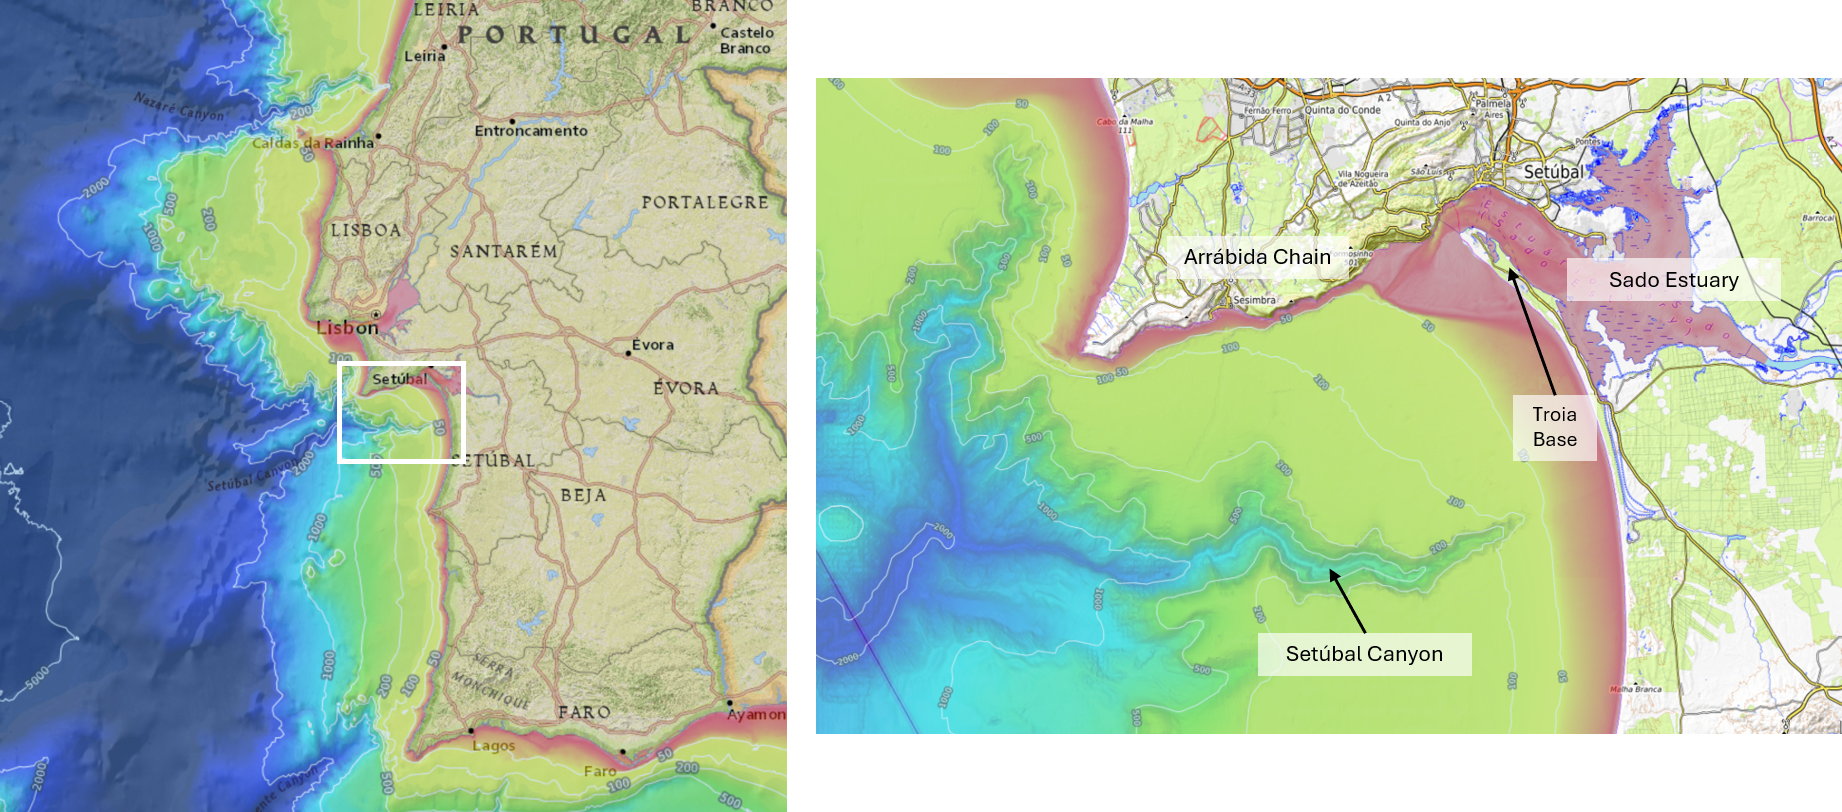
\includegraphics[scale=0.5]{fig/fig_setubal_bay.png}
  \caption{domain}
  \label{fig:domain}
\end{figure}


%\begin{figure}[!h]
 % \vspace{-0.5cm} \centering \subfigure[Map of Portugal and the study
 % area highlighted with the red
%  rectangle.]{\label{fig:po-map}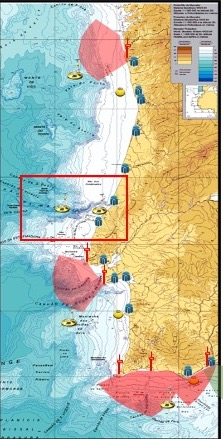
\includegraphics[scale=0.5]{fig/po-map.jpeg}}
 % \hspace{+0.3cm} \subfigure[Zoomed in bathymetry showing the Nazar\'e
%  canyon-Berlengas area (isobaths with depth in meters) and its
 % environment including the placement of the two
 % buoys.]{\label{fig:domain}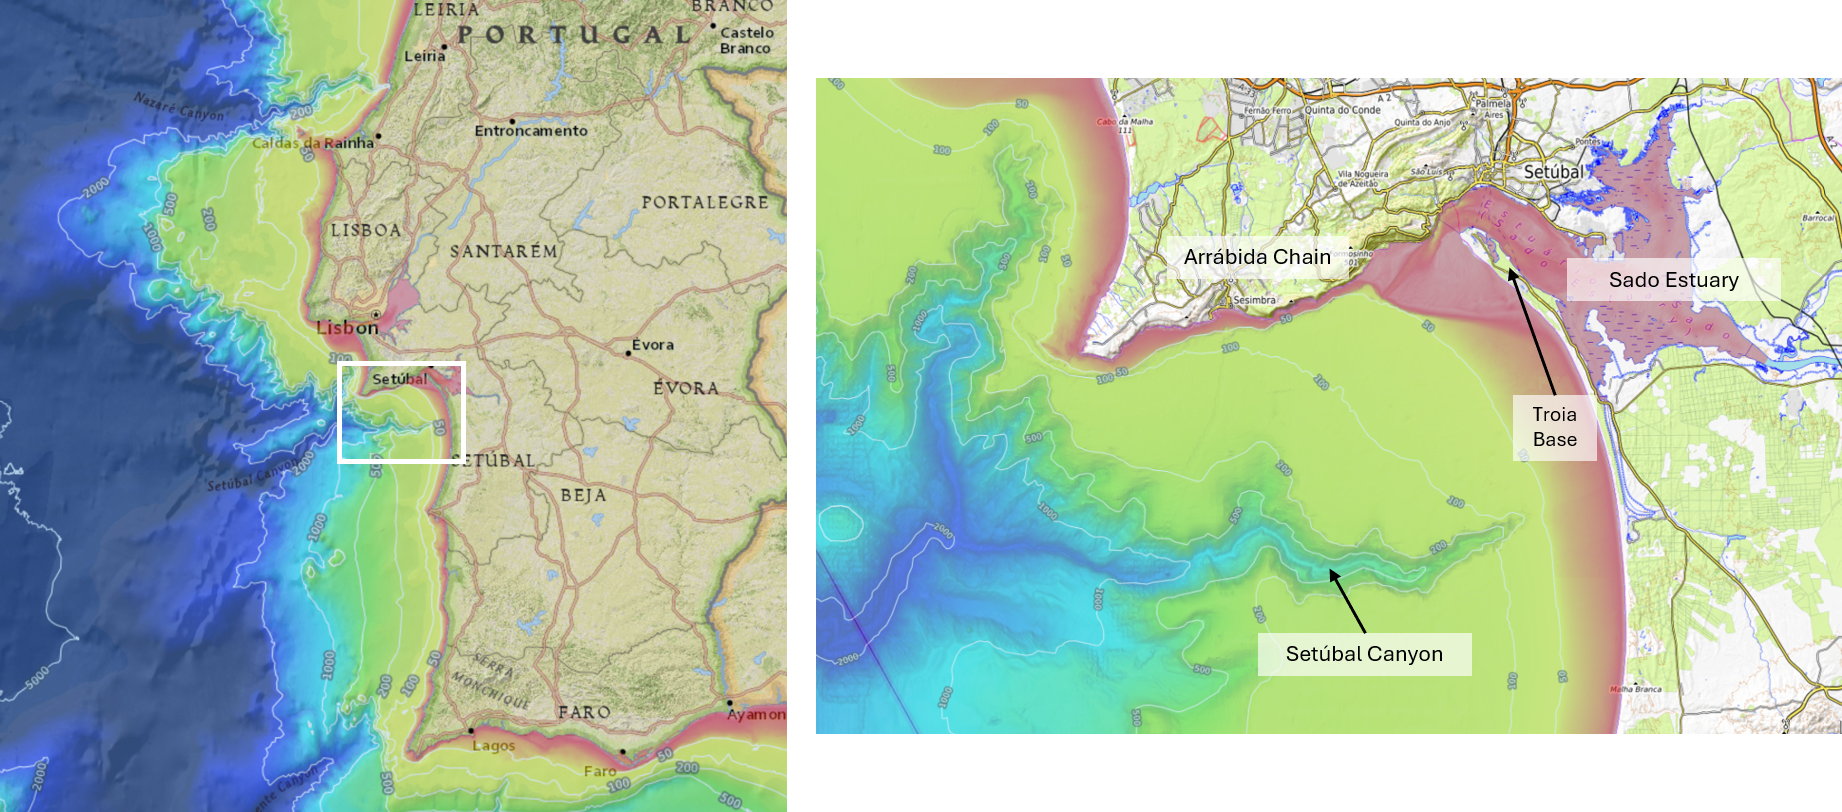
\includegraphics[scale=0.5]{fig/fig_setubal_bay.png}}
%  \subfigure[Predictions of currents and temperature at 10m depth from
 % a \texttt{HOPS} (Harvard Ocean Prediction System) model with
 % assimilation of temperature and salinity measurements collected by
 % CTD profiles and
  %current-meters.]{\label{fig:model}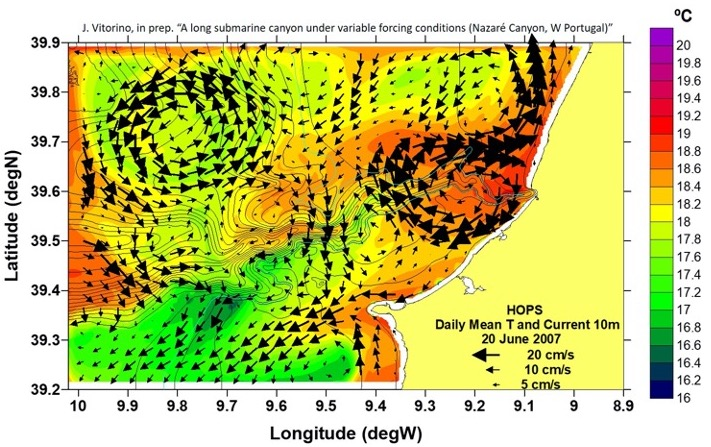
\includegraphics[scale=0.50]{fig/model.jpeg}}
  %\caption{\subref{fig:po-map} \& %\subref{fig:domain} show detailed
  %  views of the proposed study area for \proje, while
    %\subref{fig:model} shows model predictions for the dynamic region
    %driven by bathymetry and %external forcing.}
%  \label{fig:studyarea-1}
%\end{figure}


\begin{figure}[!h]
  \vspace{-0.5cm}
  \centering
  \subfigure[]{\label{fig:chlshelf}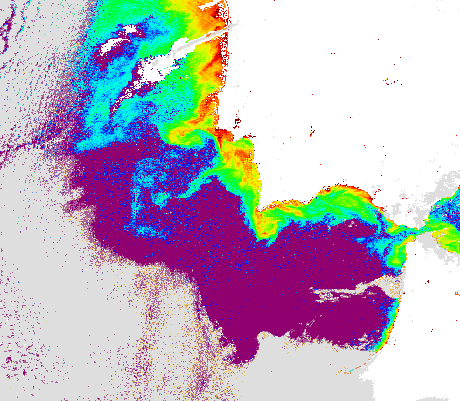
\includegraphics[scale=0.45]{fig/chl-shelf.png}}
  \subfigure[]{\label{fig:chldomain}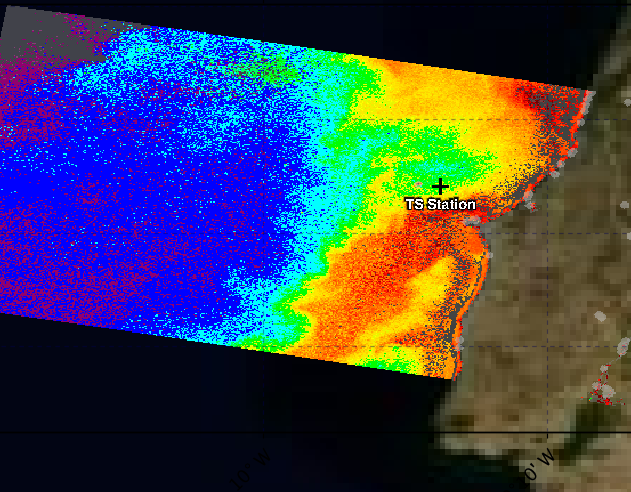
\includegraphics[scale=0.4]{fig/chl-domain.png}}
  \subfigure{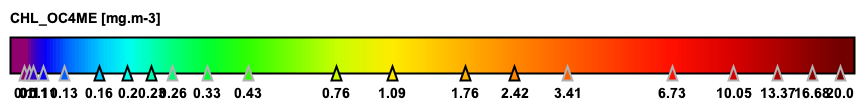
\includegraphics[scale=0.3]{fig/legend.png}}
  % \hspace{+0.3cm} 
  \subfigure[]{\label{fig:tmpchange}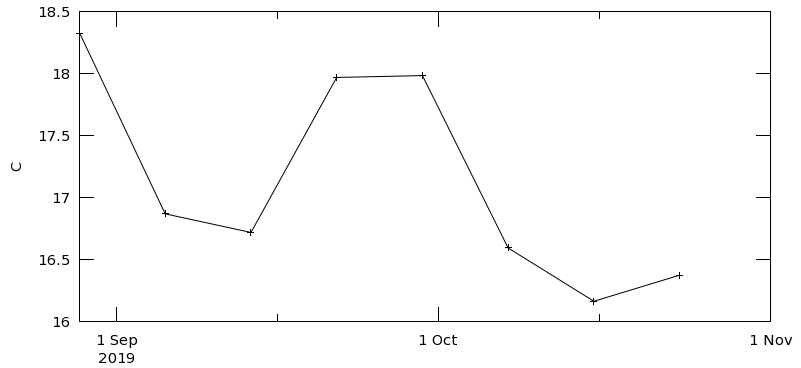
\includegraphics[scale=0.285]{fig/temp-change.png}}
  \subfigure[]{\label{fig:chlchange}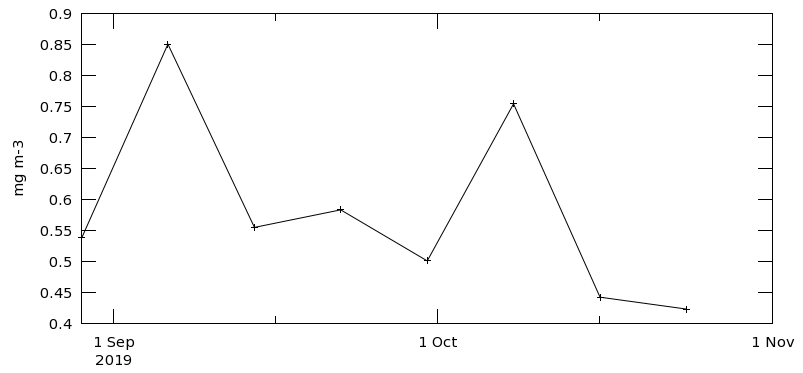
\includegraphics[scale=0.285]{fig/chl-change.png}}
  \caption{300m resolution remote sensing images from Sentinel 3 from
    September 6\textsuperscript{th} 2019 showing along shelf
    \subref{fig:chlshelf} and zoomed in Chlrophyll filaments
    \subref{fig:chldomain} emanating from the proposed study area of
    Nazar\'e canyon-Berlengas. \subref{fig:tmpchange} and
    \subref{fig:chlchange} show time series with rapid changes of
    temperature and chlorophyll respectively in the area.}
  \label{fig:studyarea-2}
\end{figure}

\section*{Logistical and budgetary information}


% Off shore in the Nazar\'e canyon-Berlengas area are two islands of
% Berlengas and Farilho\~es part of a protected nature preserve. With
% special permission we expect to be able to be based in Berlengas for a
% period of 3 weeks to conduct off shore operations. A small team will
% also be present onboard the \inst research vessel where if needed,
% deployment and recovery of assets well off shore at the boundaries of
% the survey region, can be done. In addition \inst will be in a
% position to provide a RHIB or a rigid boat for near-shore operations
% from the two islands.

% \univ will provide the bulk of the robotic assets including aerial,
% surface and underwater vehicles as also the team to operate them. The
% team will be split between being based in Berlengas, the research
% vessel and also provide remote monitoring from Porto. \univ will
% provide at least one glider to operate outside the shelf to augment
% model observations in the meso-scale.

Our approximate and highly leveraged budget for this exercise is
expected to be \textbf{$\sim \$100$ K to support this 21 day (3 week)}
operation. This includes all robotic vehicles, faculty and staff from
all the partner organizations, transportation of assets and people in
Portugal as also insurance and communication costs for and during the
exercise. The budget will directly support software development to
extend observation quality control, assimilation and ML based
approaches to entropy reduction in modeling, all based out of \unive.


\paragraph{Roles and responsibilities} \univ will be the lead
organization, provide aerial, surface and underwater vehicles,
communication equipment and command/control software while
coordinating all activities. Funding requested will primarily support
students and staff in Porto and Lisbon for software development, model
development and operations.  \colo will work on making bio-optical and
biological measurements and providing analysis and data to augment
\ulis modeling. Table \ref{tab:roles} summarizes the roles and
contributions of all partners.

\begin{table}[!t]
  \centering
  \vspace{-0.5cm}
  \begin{tabular}{|p{1.5cm}|p{10cm}|p{4cm}|}\hline 
    \rowcolor{Gray}
    \bfseries Inst. &\bfseries Role &\bfseries Contributions\\
    \hline
    \univ & Lead organization, CONOPS (concept of operations) design and
            implementation, software engineering, reporting, experiment design, outreach
                                    &aerial/surface/underwater
                                      vehicles, comms, gliders, operations team\\
    \hline
    \ulis & Physical Oceanography, Modeling, observation assimilation,
            prediction, Modeling, Machine Learning and entropy reduction&
                                                                          outreach\\
    \hline
    \colo & Ocean dynamics, sampling algorithms&\\
    \hline
  \end{tabular}
  \caption{Roles and responsibilities and in-kind contributions in
    \proj for the proposed 2021 Sept-Oct field experiment. All team
    members will be collaboratively involved in experiment design and
    post experiment publishing.}
  \label{tab:roles}
\end{table}

\paragraph{Operational Considerations} While most experiments in the
coastal zone rely on ship-board measurements and gliders, the
challenging nature of this high-energy environment requires a mix of
assets in addition to gliders. Currents can be in the region of
$\sim 2$ knots, there is substantial variability in the upper
water-column and with high primary productivity and the existence of
coastal upwelling to provide for a rich nutrient base and the study
region has a robust presence of fishermen, nets and crab pots. We
expect to field an ensemble of low cost robotic vehicles including
propelled AUVs, unmanned surface vehicles, low cost Lagrangian
profilers and aerial vehicles with RGB and potentially hyper-spectral
imaging sensors. Accessibility to the two islands will also provide
some shelter from weather for continuous operations including rapid
launch/recovery of in-situ assets. In addition, we will obtain images
from the \textbf{SeaHawk} nano-satellite (developed with funding from
the Moore Foundation when Subramaniam was program director there) with
a high quality multi-spectral
imager~\footnote{\url{https://uncw.edu/socon/index.html}}. Finally,
\univ has a number of low cost temperature/density sensors which when
calibrated with CTDs on the vessel and robotic vehicles, will enable
local fisherman to provide timely data in this meso-scale
region. % All such data will be assimilated into the ocean models run by
% \inst and supported by \mit which continues to support \texttt{HOPS}
% development.

% \paragraph{COVID protocol} As per standard oceanographic cruise
% protocol in current circumstances, we will follow the guidance of WHO
% and the US CDC; all personnel will isolate 5 days before the
% experiment after appropriate PCR tests for safety and stay in one
% pod. Those onboard the \inst research vessel will follow Portuguese
% Navy guidelines and also isolate prior to the cruise and have no
% contact with shore based personnel during the course of the
% experiment.

\section*{Outreach}

% \inst has had continued and extensive engagement over the years with
% the local authorities including the Nazar\'e city officials and local
% fishermen. As a result we will engage the fishing community to carry
% our low cost temperature/density sensors and also help provide access
% to the team to be able to commute to the islands when necessary,
% subject to health protocols.
In addition, we expect to engage local high school students prior and
after the experiment, to entice them into thinking about careers in
science and technology, much as we have done in the past with success
in another \org funded
program~\footnote{\url{https://sunfish.lsts.pt/en/outreach/education}}. In
\oldproj for instance, we engaged a local science high school with the
participation of the district's superintendant. 

With the world-wide interest in the area \proj will also work with the
local authorities to showcase our work in Portuguese and English
language media outlets.

Finally, publications resulting from the project will be targeted
towards peer-reviewed journals including \emph{Oceanography, Science
  Robotics, IEEE Transactions on Field Robotics, Int. J. of Robotics
  Research, AI Journal, Autonomous Robots, PLOSone, Frontiers} and
high-impact conferences such as \emph{AAAI, IJCAI, ISER, ICAPS, RSS,
  IROS, ICRA and IEEE AUV} where we have frequently published.

